\documentclass[aspectratio=169]{beamer}
\usepackage{tikz}
\usepackage{array}
\usepackage{multimedia}
% numbering=none,counter,fraction - frame number at bottom right
\usetheme[block=fill,numbering=none,progressbar=foot]{metropolis}           % Use metropolis theme

\definecolor{RoyalBlue}{cmyk}{1, 0.50, 0, 0}
\definecolor{BgBlue}{cmyk}{1, 0.5, 0,0.8}

\setbeamercolor{progress bar}{fg=RoyalBlue!100, bg=RoyalBlue!30}
\setbeamercolor{frametitle}{bg=BgBlue!100}
\title{AIOLI - AI Open Lab Initiative}
\subtitle{Digital Assistants - Alexa}
\date{\today}
\author{\texorpdfstring{\url{chriamue@gmail.com}}{Christian M\"uller}}

%%%%%%%%%%%%%%%%%%% TITLE RIGHT
\makeatletter
\setbeamertemplate{title page}{

  \begin{minipage}[b][\paperheight]{\textwidth}

    %\centering
    \raggedleft
    \ifx\inserttitlegraphic\@empty\else\usebeamertemplate*{title graphic}\fi
    \vfill%
    \ifx\inserttitle\@empty\else\usebeamertemplate*{title}\fi
    \ifx\insertsubtitle\@empty\else\usebeamertemplate*{subtitle}\fi
    %\usebeamertemplate*{title separator}
    \ifx\beamer@shortauthor\@empty\else\usebeamertemplate*{author}\fi
    \ifx\insertdate\@empty\else\usebeamertemplate*{date}\fi
    \ifx\insertinstitute\@empty\else\usebeamertemplate*{institute}\fi
    \vfill
    \vspace*{1mm}
  \end{minipage}
}

\setbeamertemplate{title}{
  \raggedleft%
  \linespread{1.0}%
  \inserttitle%
  \par%
  \vspace*{0.5em}
}
\setbeamertemplate{subtitle}{
  \raggedleft%
  \insertsubtitle%
  \par%
  \vspace*{0.5em}
}
\makeatother

%%%%%%%%%%%%%%%%%%%%%%%

\begin{document}


{\usebackgroundtemplate{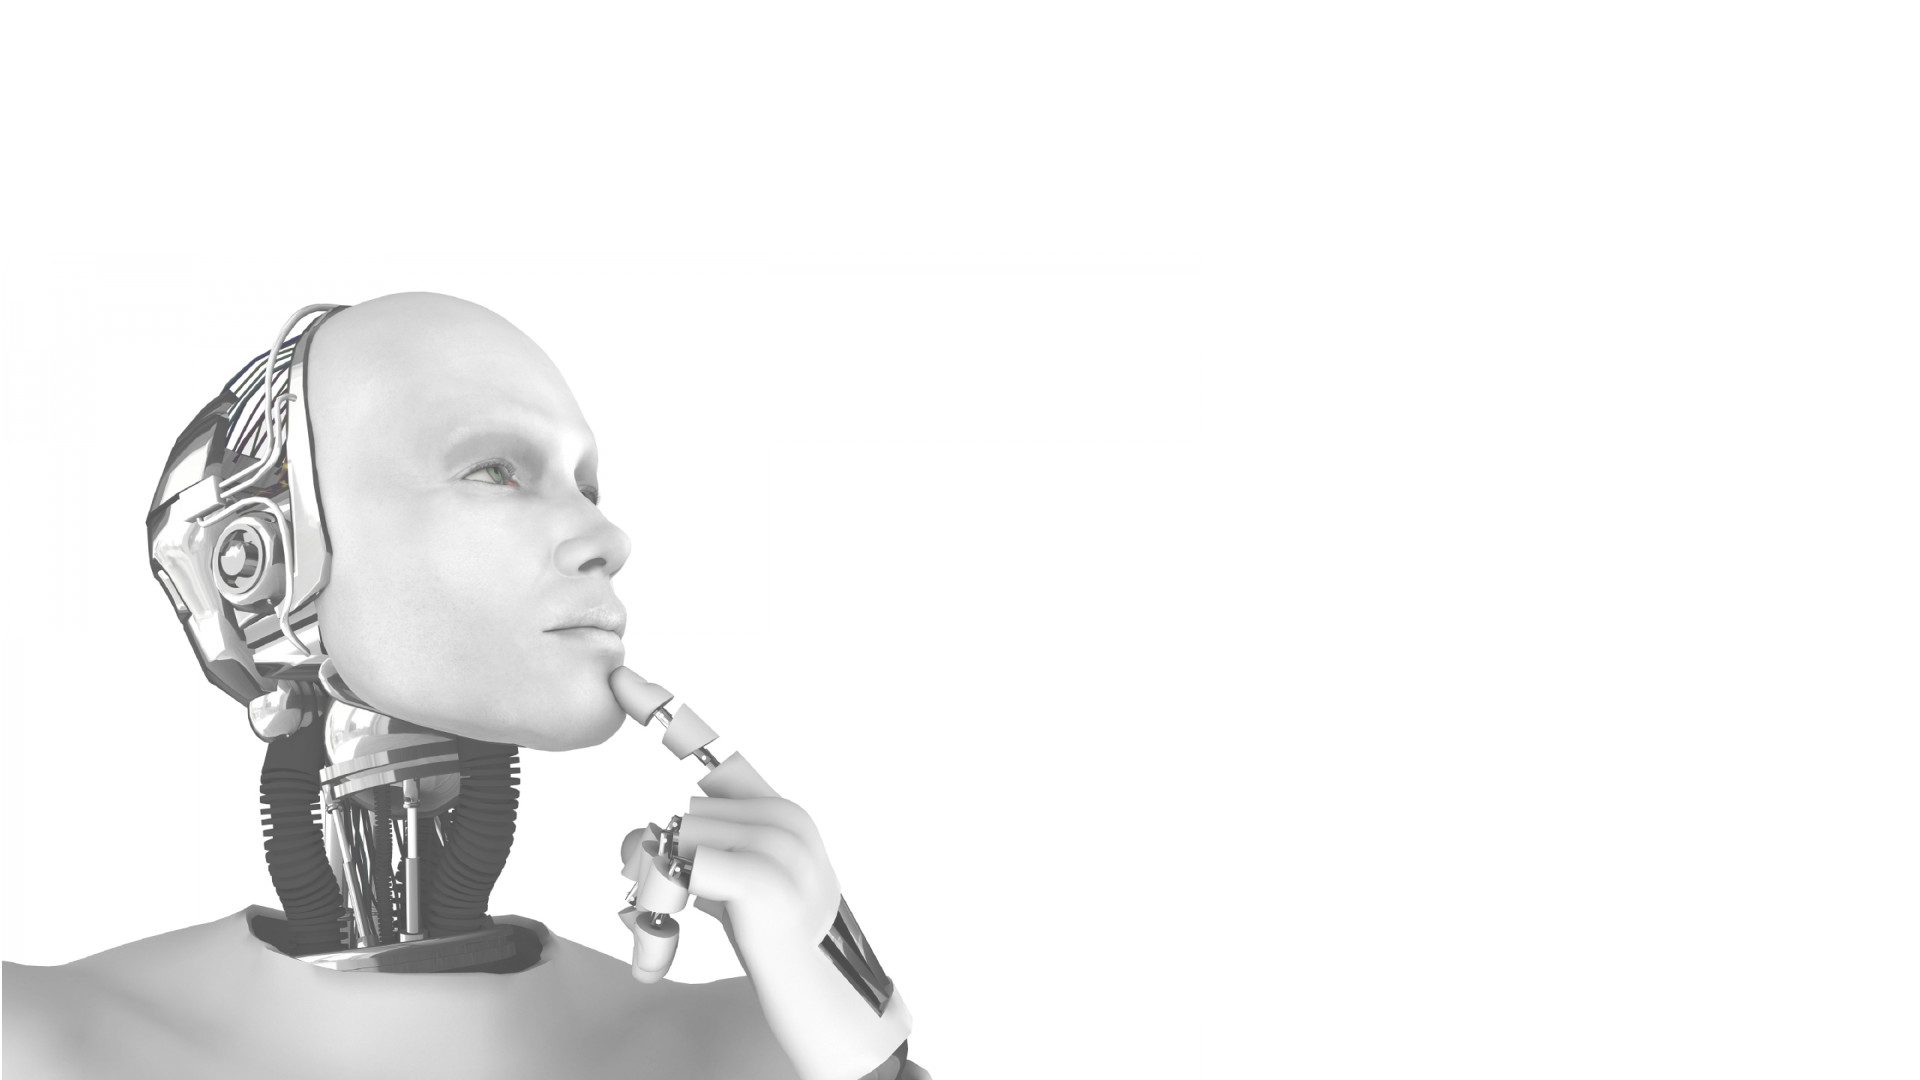
\includegraphics[width=\paperwidth]{images/ai_bg.jpg}}
\maketitle}

%\usebackgroundtemplate{
%}

%%%%%%%%%%%%%%%%%%%%%%%%%%%%%%%%%%%%%%%%%%%%%%%%%%%%%%%%%%%%%%%%%%%%%%%%%%%%%%%%
%                       DEFINITIONS
%%%%%%%%%%%%%%%%%%%%%%%%%%%%%%%%%%%%%%%%%%%%%%%%%%%%%%%%%%%%%%%%%%%%%%%%%%%%%%%%
%\section{SciFi debunked - Slaugherbots}
	\begin{frame}{Agenda}
		\tableofcontents
	\end{frame}


\section{Assists overview}
        \begin{frame}{List of some available assistants}
        	\centering
        	\begin{itemize}
        		\item Amazon Alexa {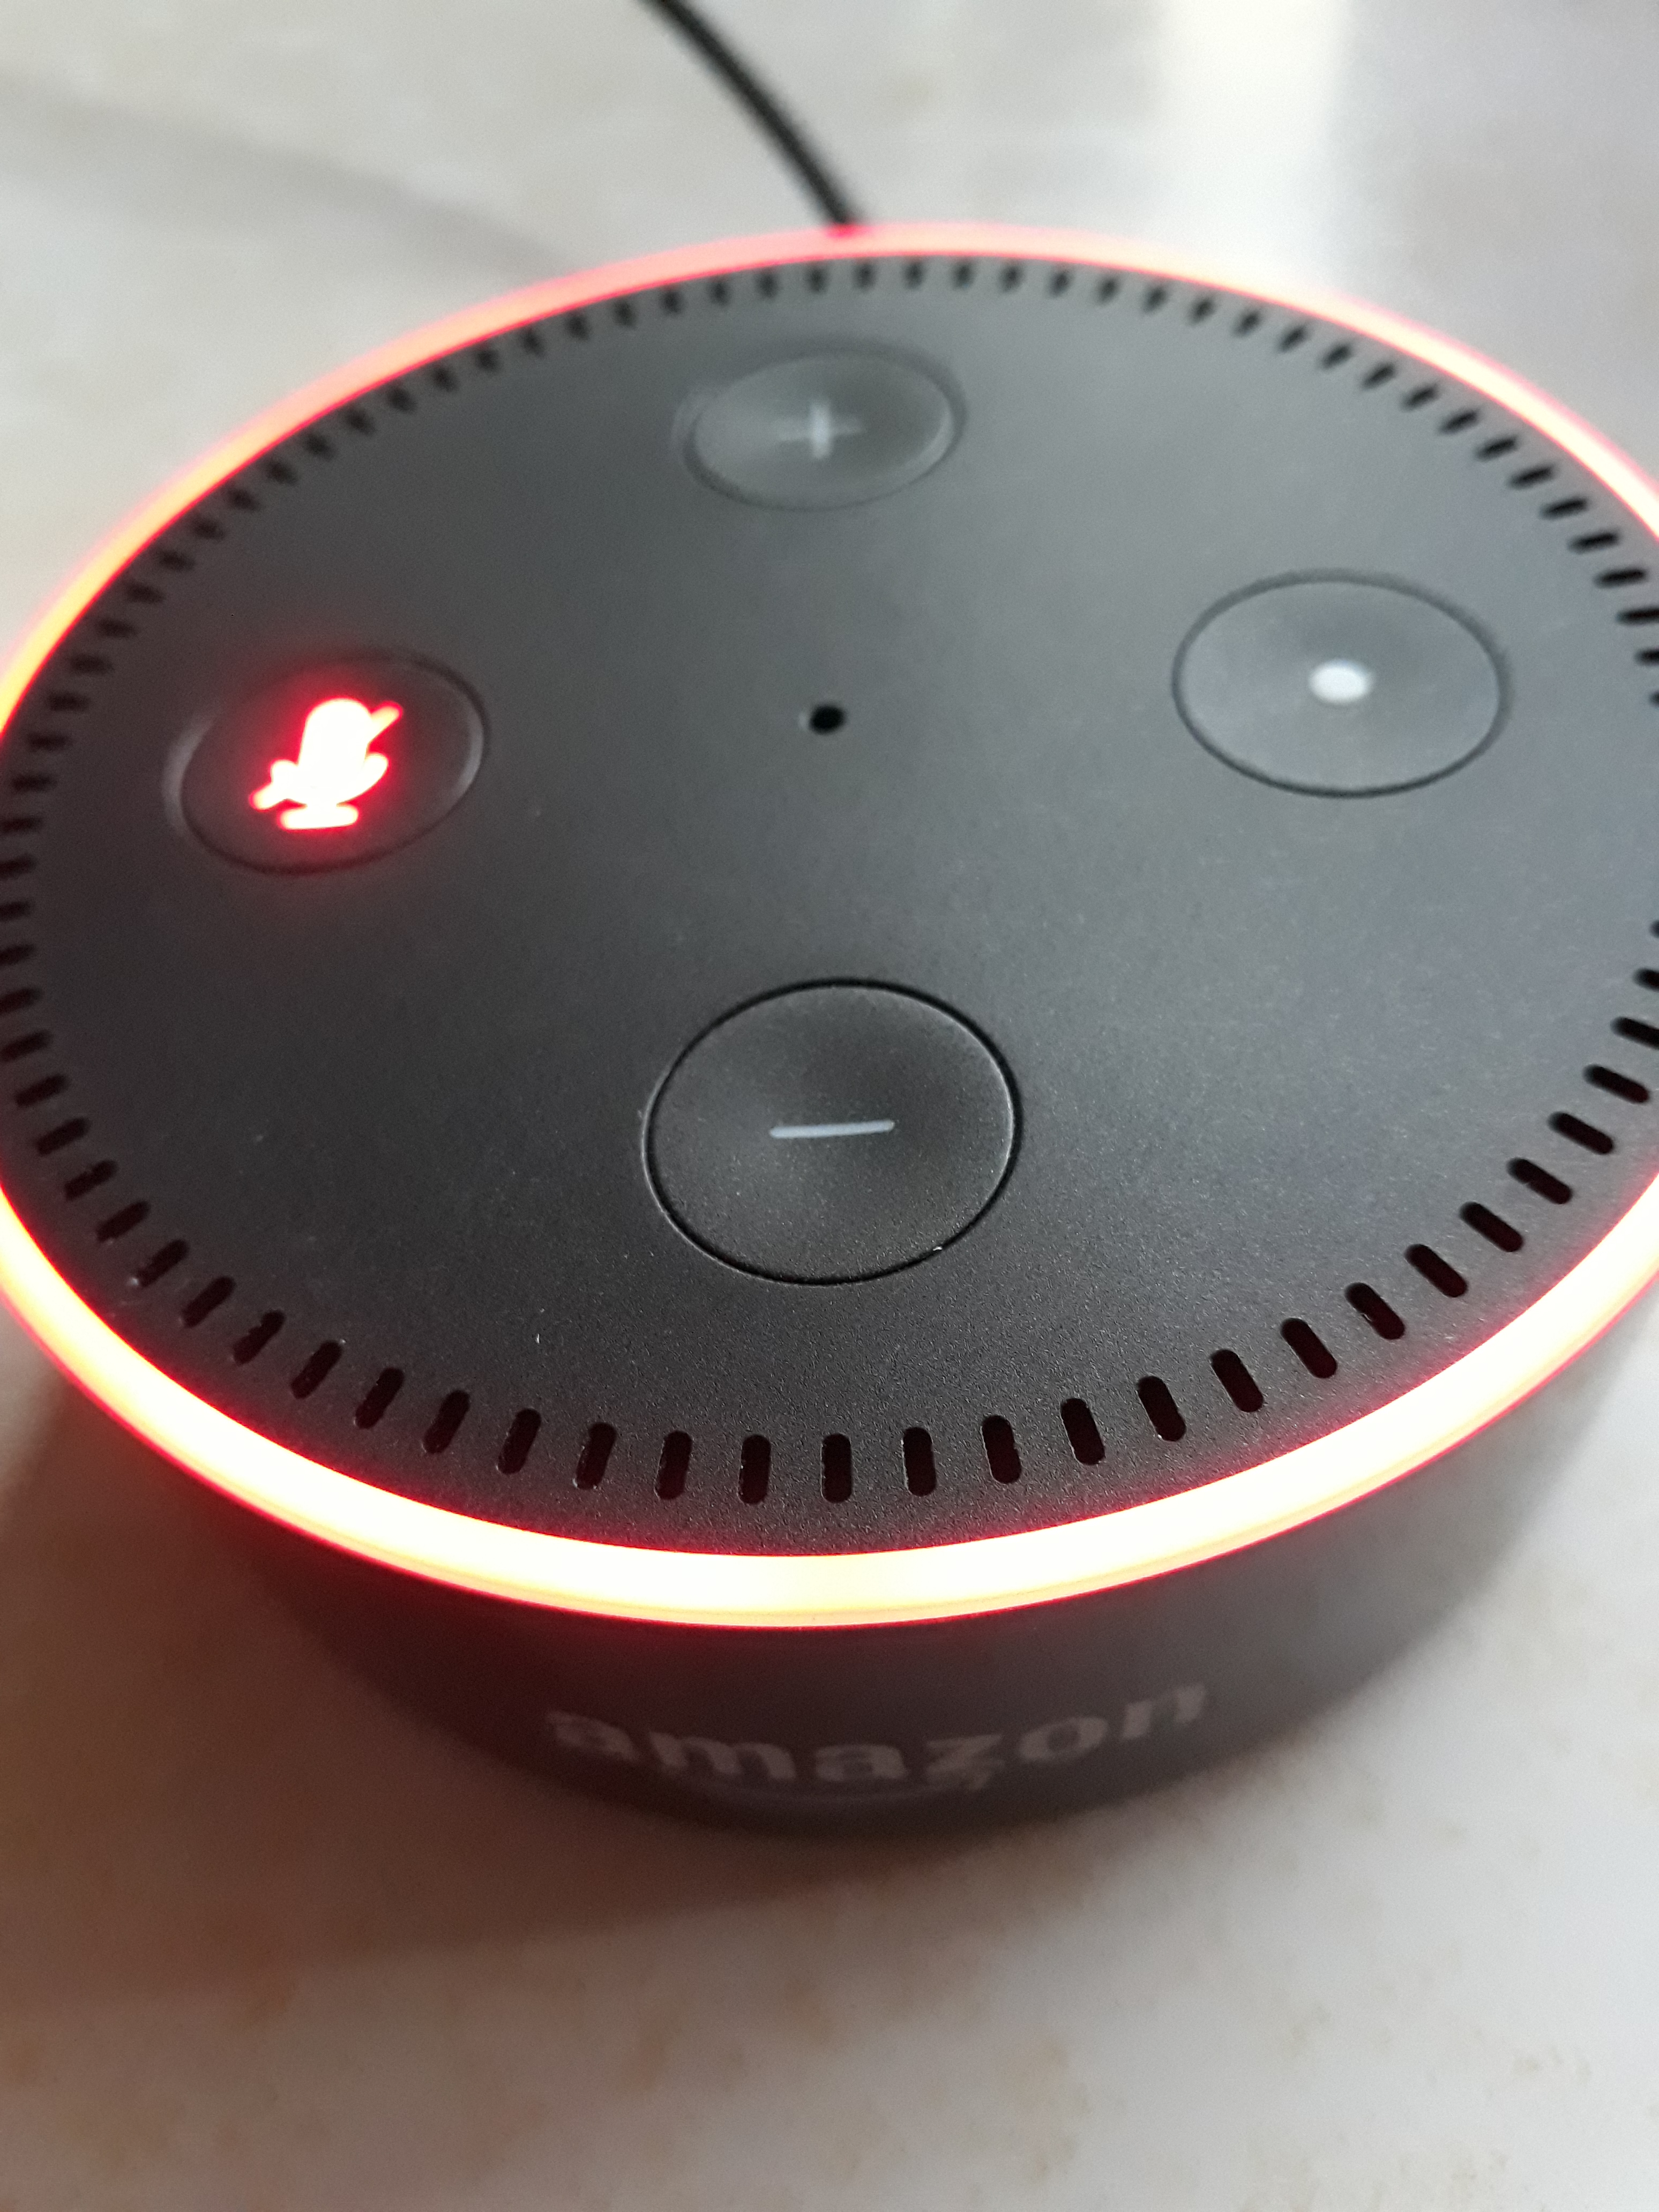
\includegraphics[width=.15\linewidth]{images/alexa_muted}}
        		
        		\item Google Home {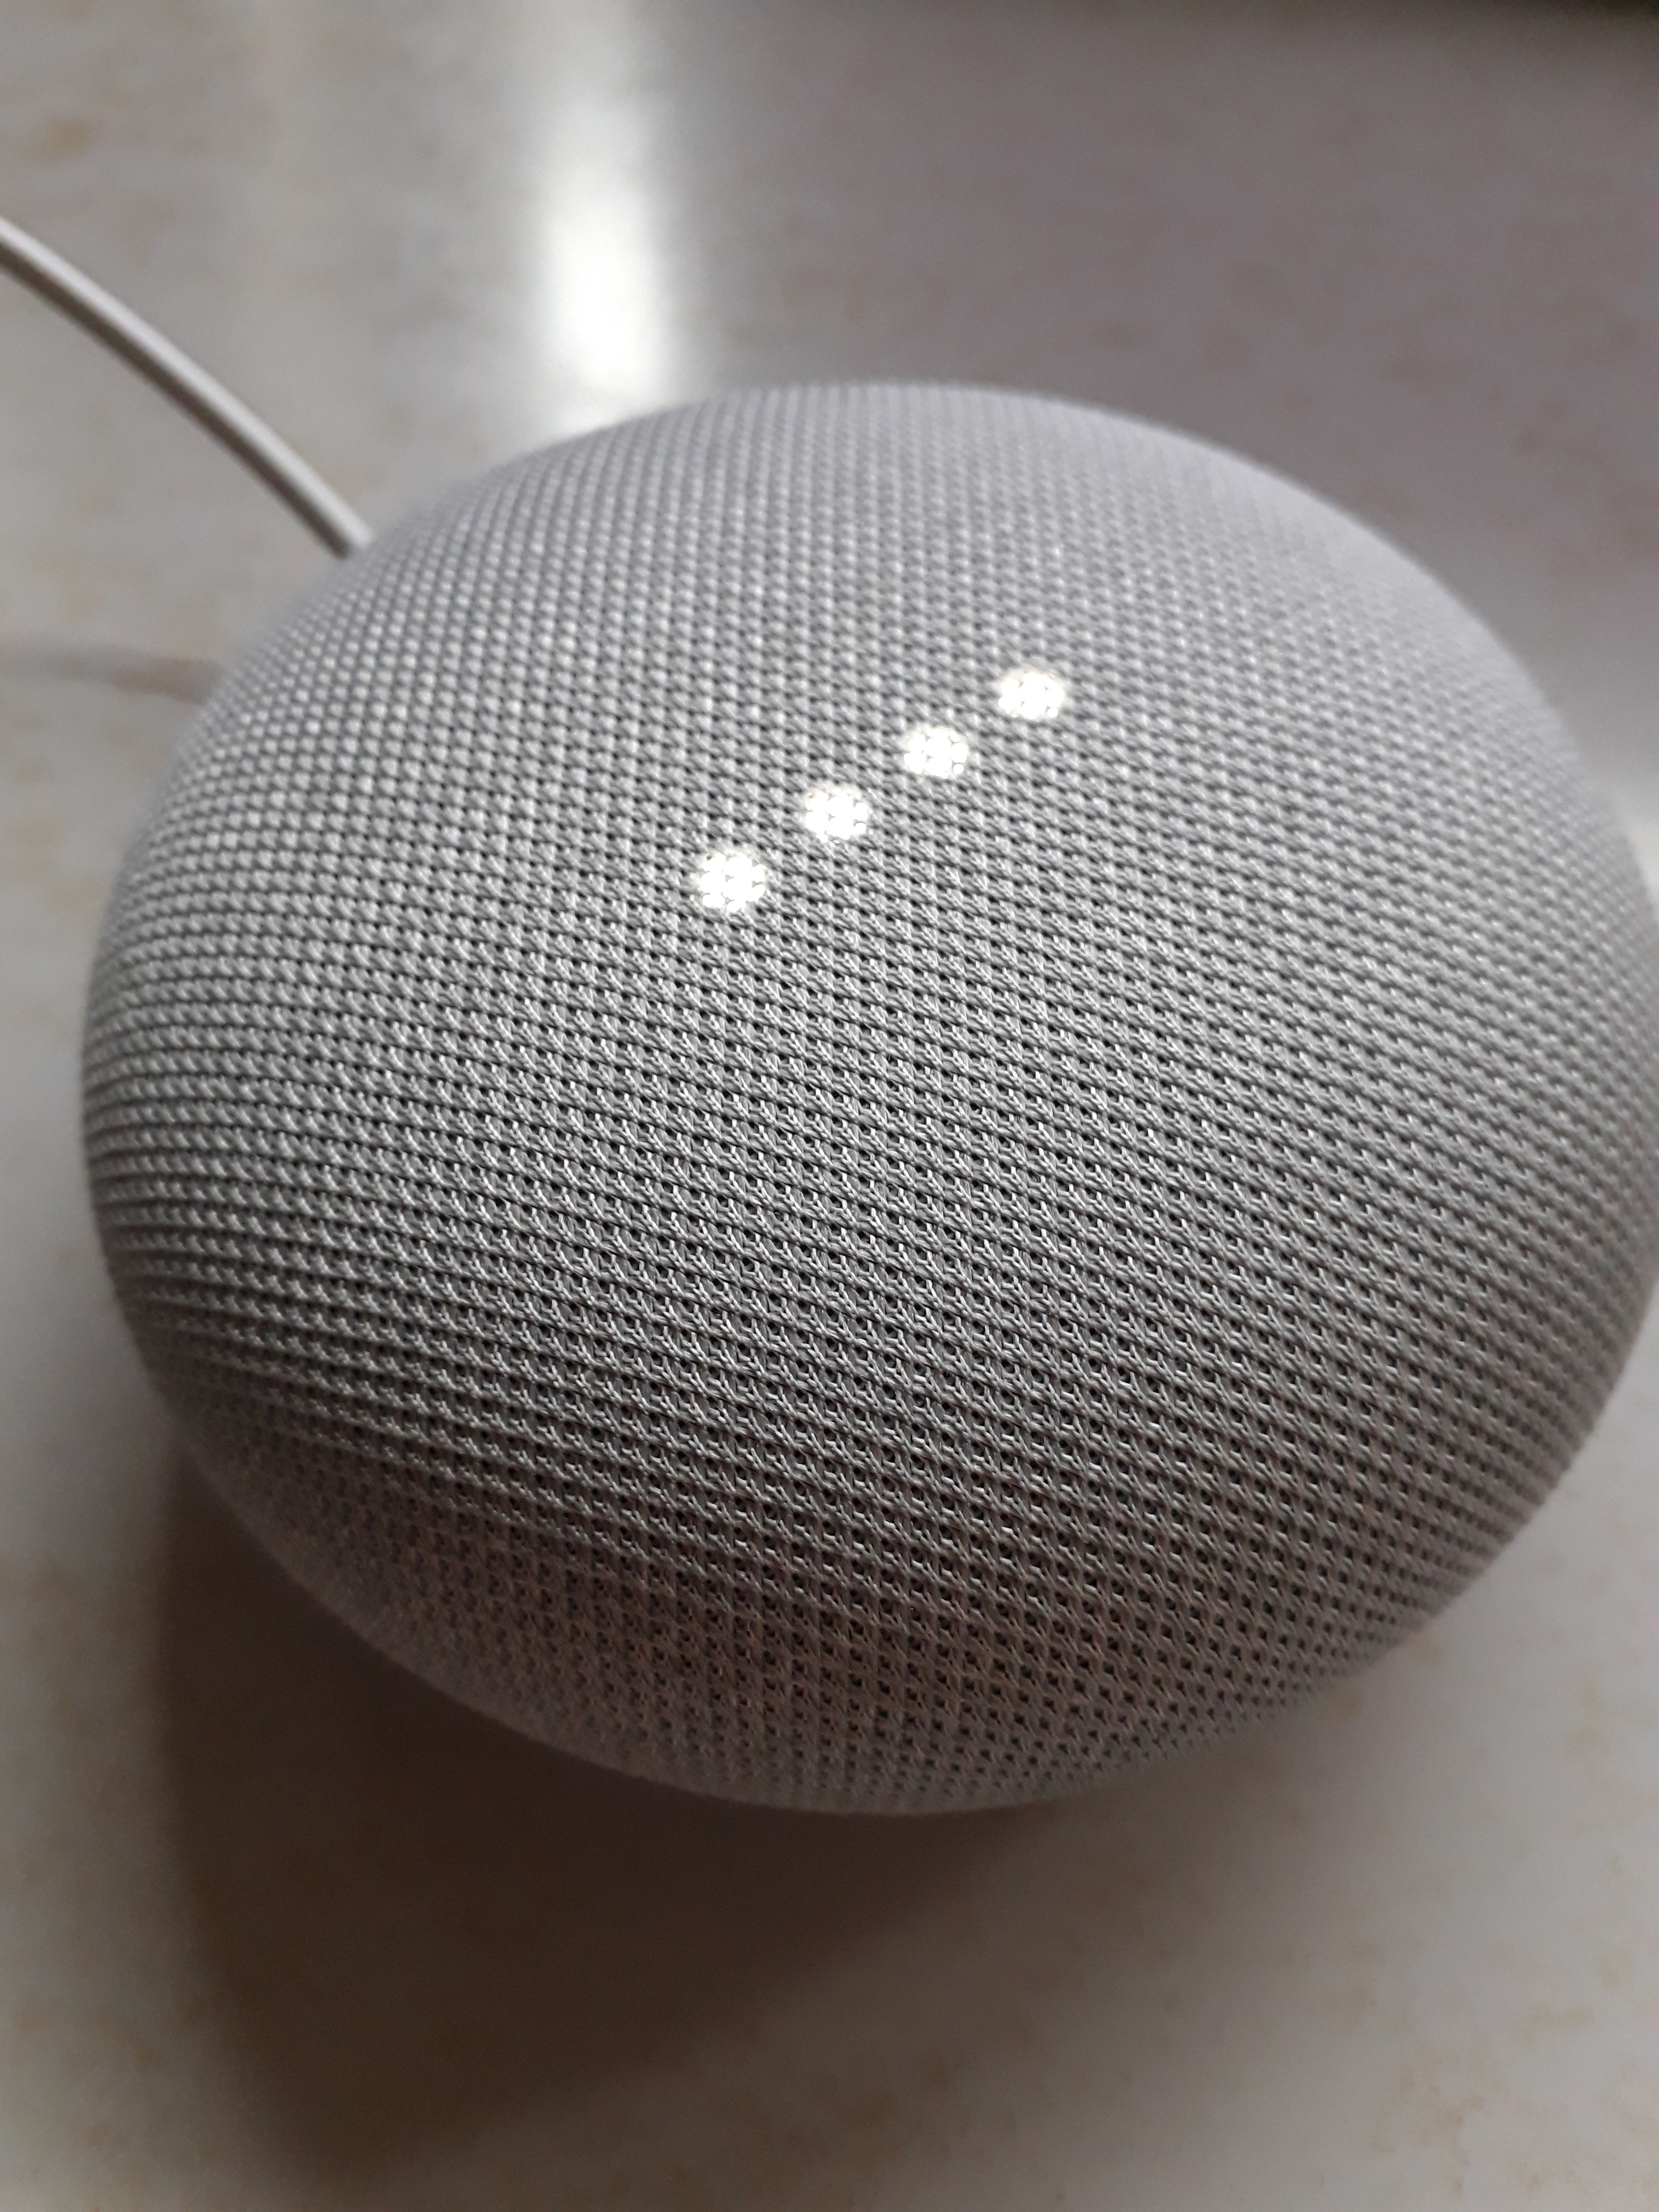
\includegraphics[width=.15\linewidth]{images/ghome}}
        		
        		\item Apple Siri
        		
        		\item Microsoft Cortana
        		
        	\end{itemize}
            
        \end{frame}

        \begin{frame}{What are they good for?}
        \centering
        \begin{itemize}
        	\item Check my Calendar
        	
        	\item Play some music
        	
        	\item Give me the news
        	
        	\item Tell me how the weather will be
        	
        	\item Make me a shopping list
        	
        \end{itemize}
     \end{frame}
 
 \begin{frame}{What are they good for? - Not much!}
 \centering
 	 	But Alexa has Skills!
 	 	
\includegraphics[width=0.8\linewidth]{images/alexadance}
\end{frame}

\section{Alexa Skills technology}
\begin{frame}{Technology}
	\begin{figure}
		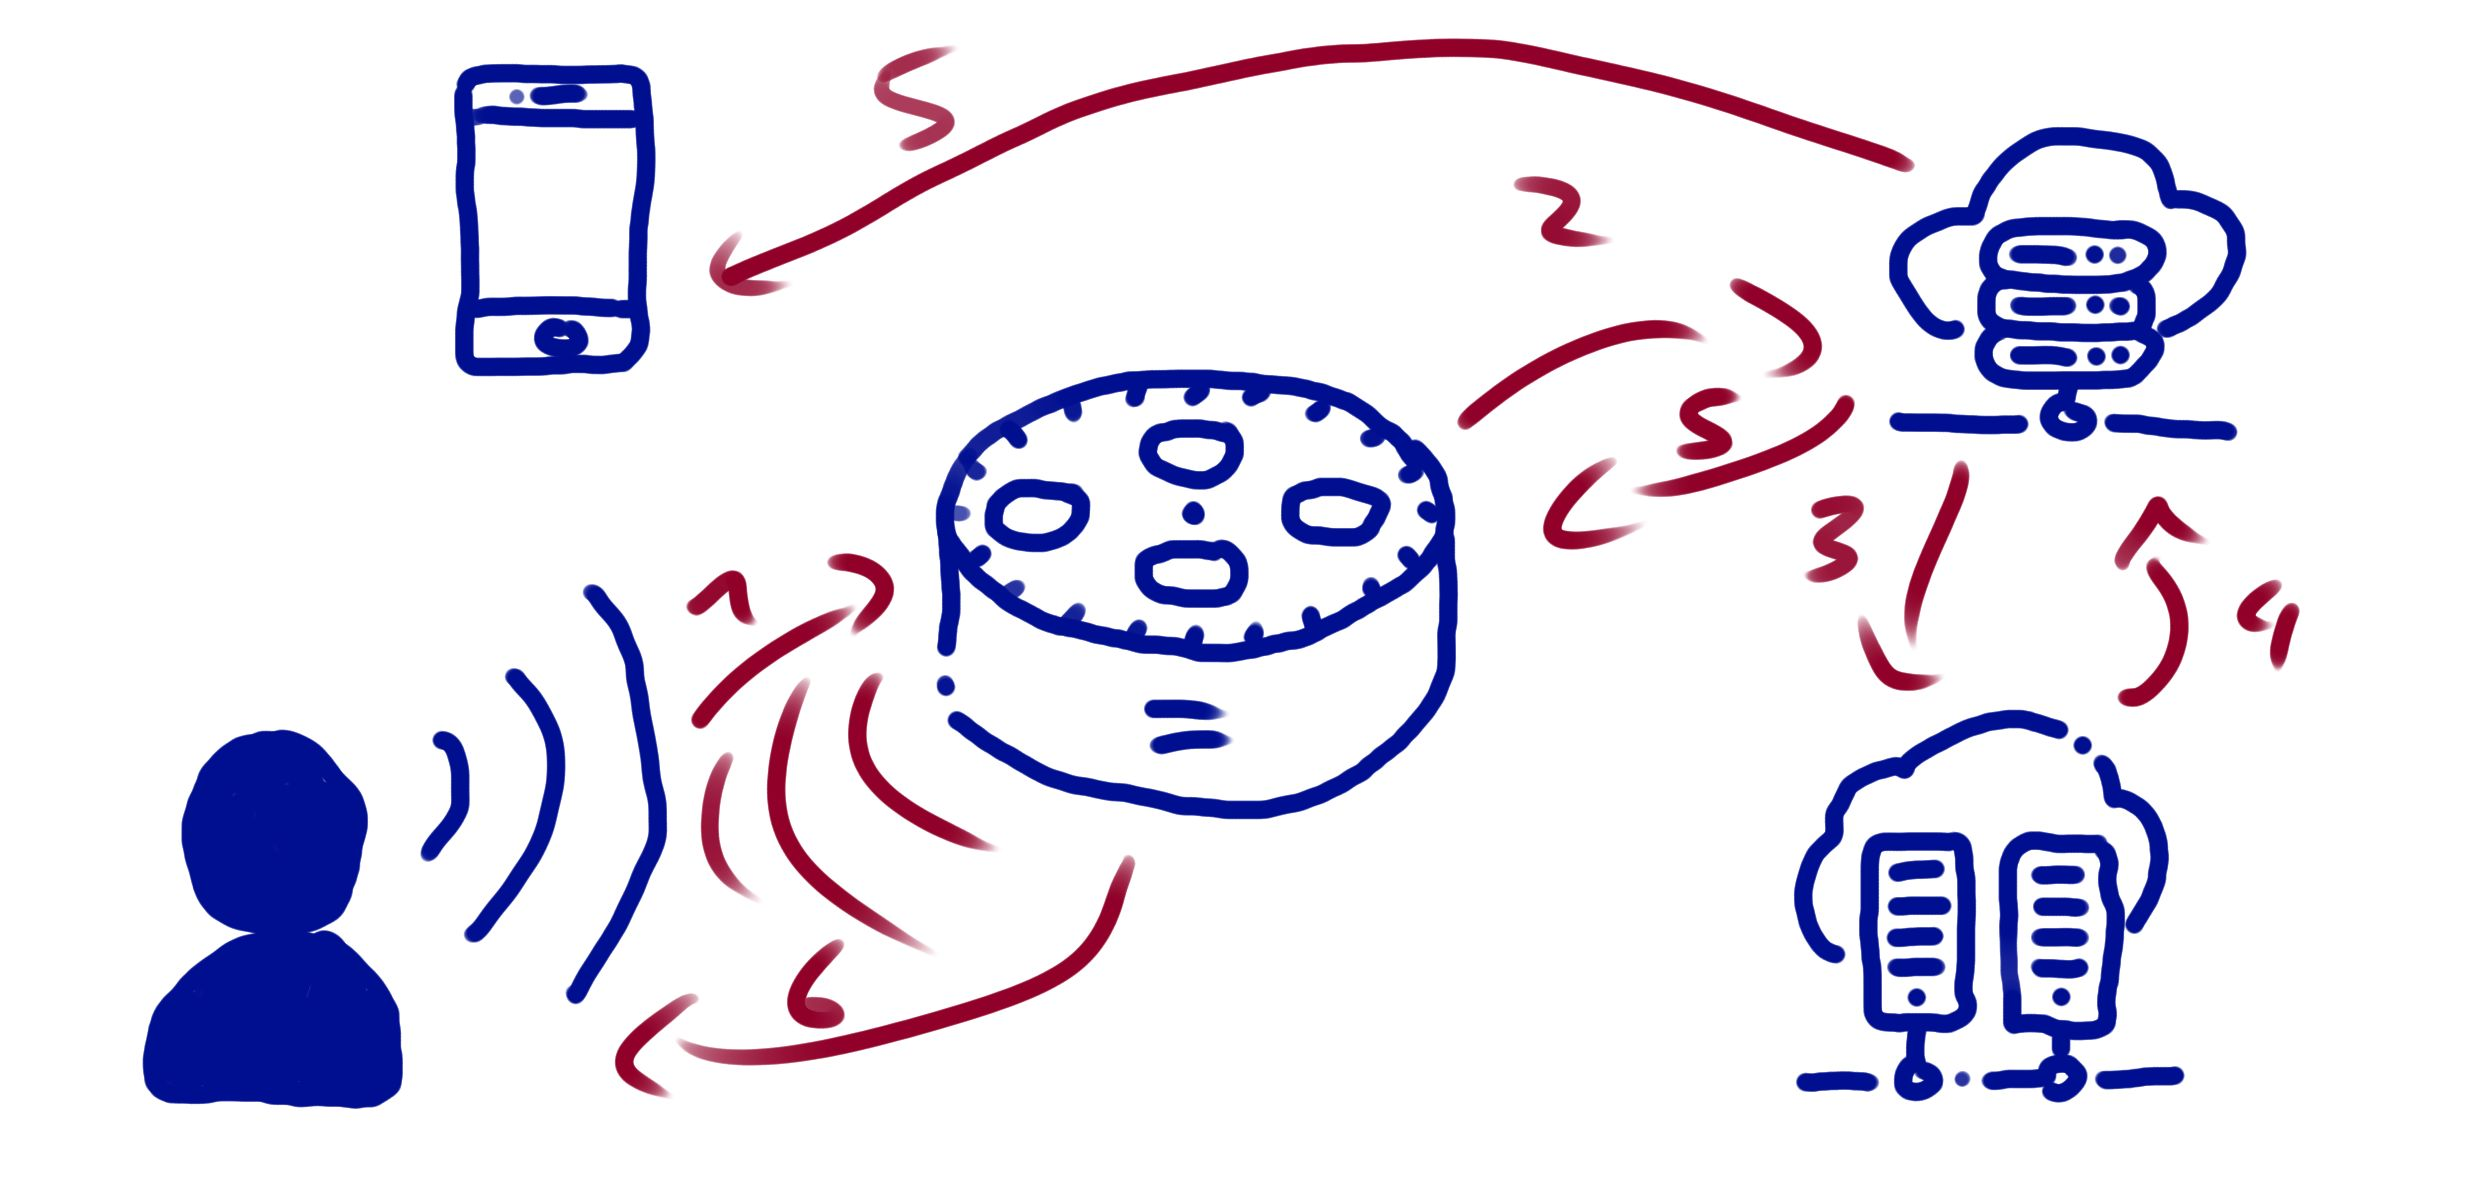
\includegraphics[width=1\linewidth]{images/alexatech}
	\end{figure}
\end{frame}

\begin{frame}{Technology}
\begin{figure}
	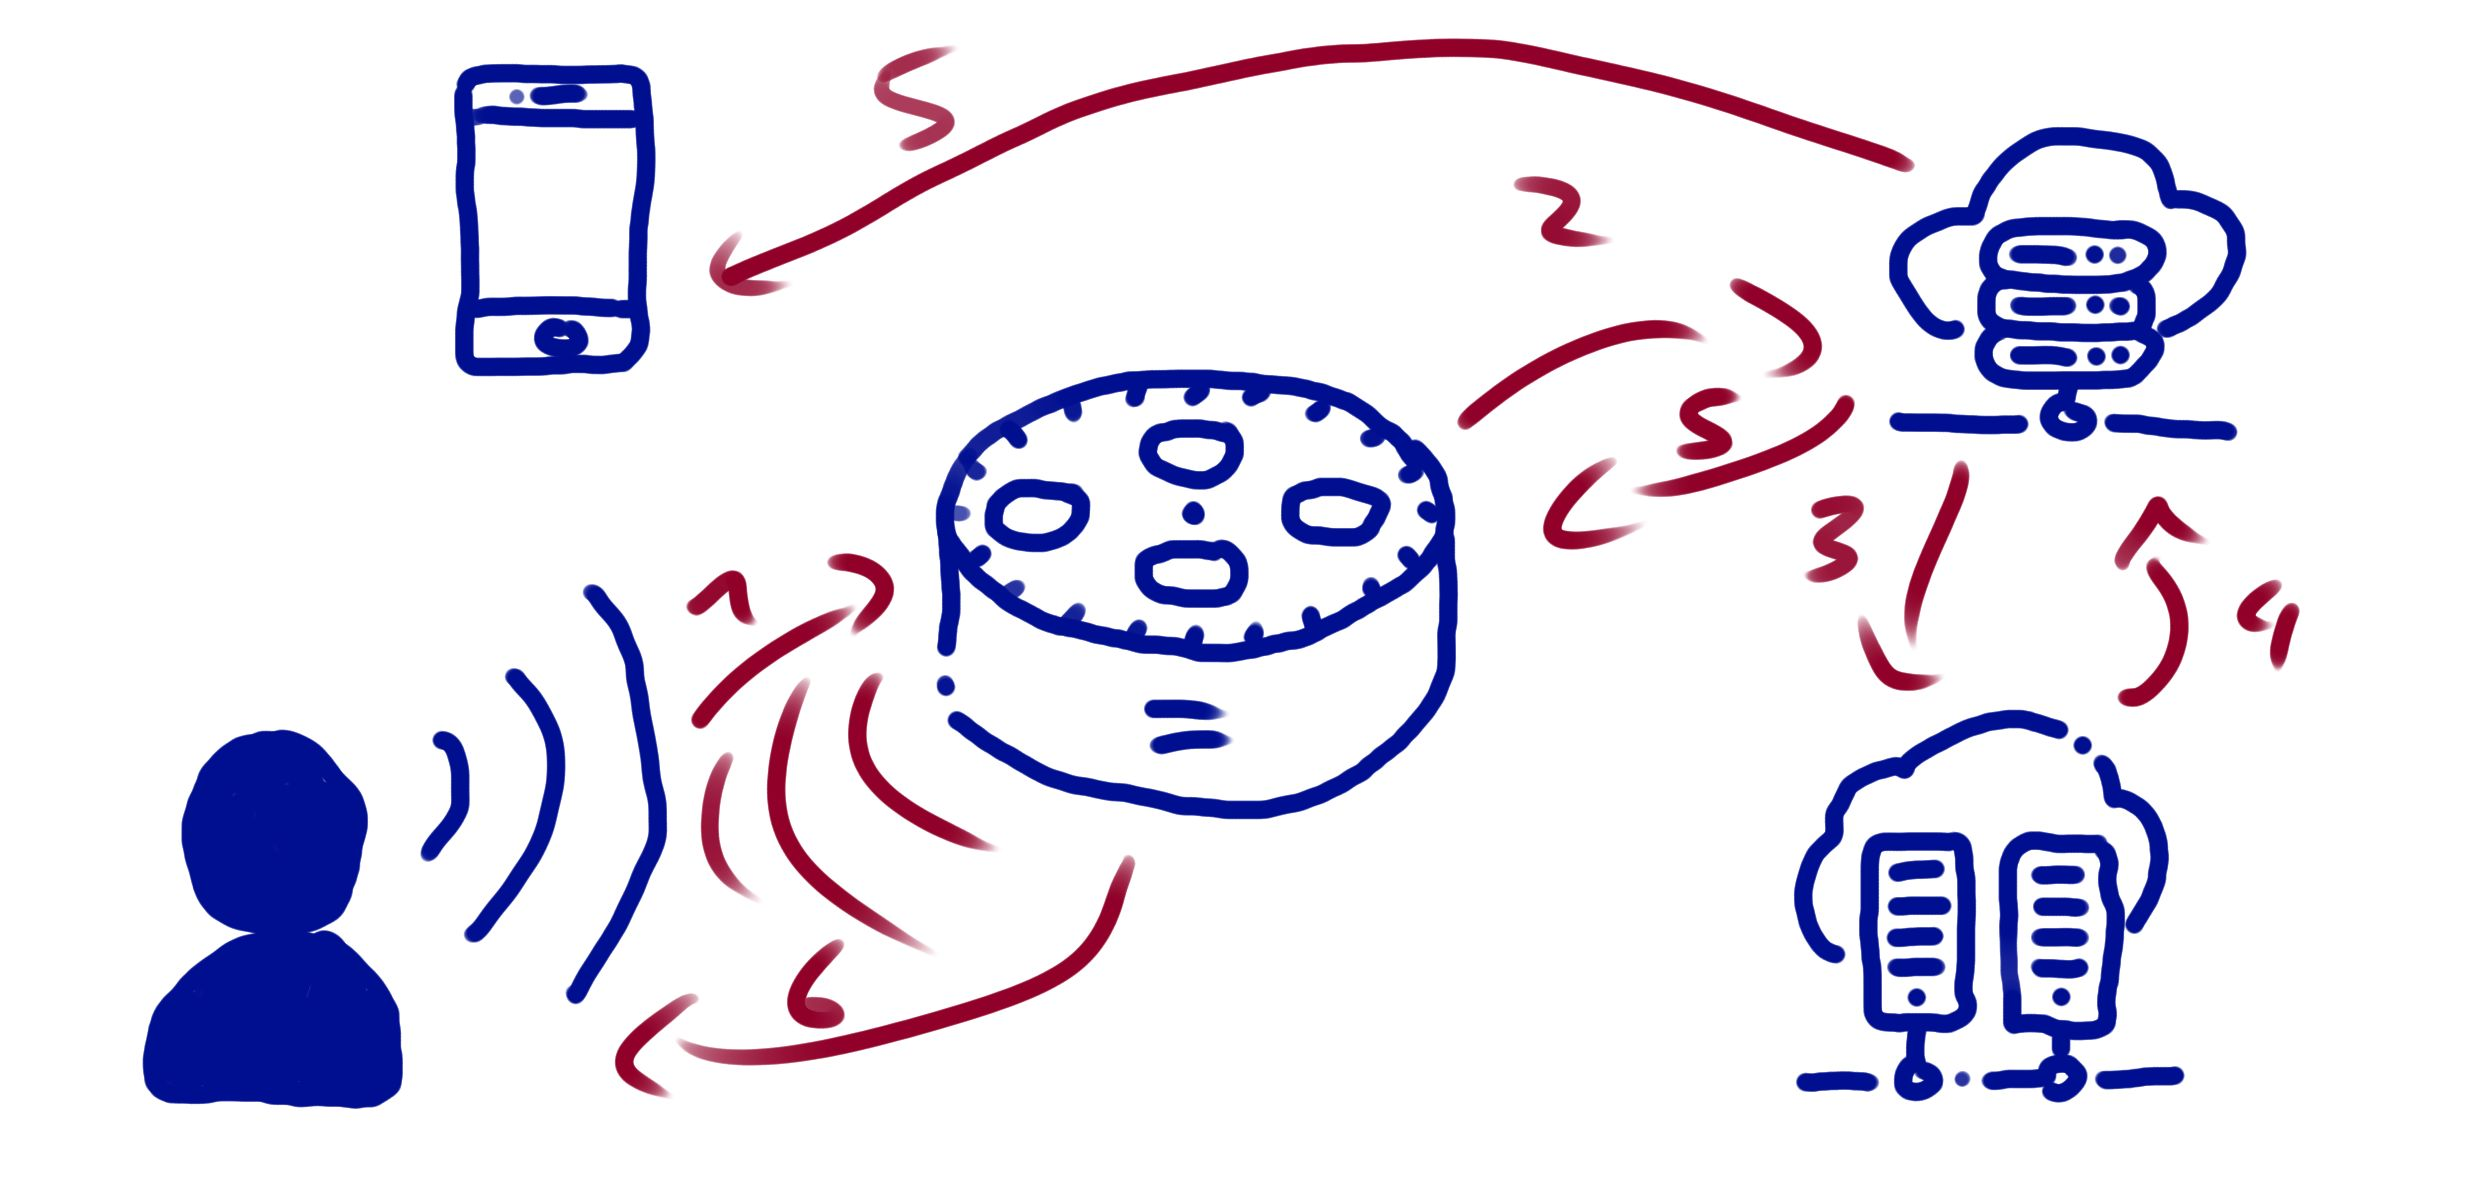
\includegraphics[width=0.9\linewidth]{images/alexatech}
\end{figure}
1. Speak to Alexa
\end{frame}

\begin{frame}{Technology}
\begin{figure}
	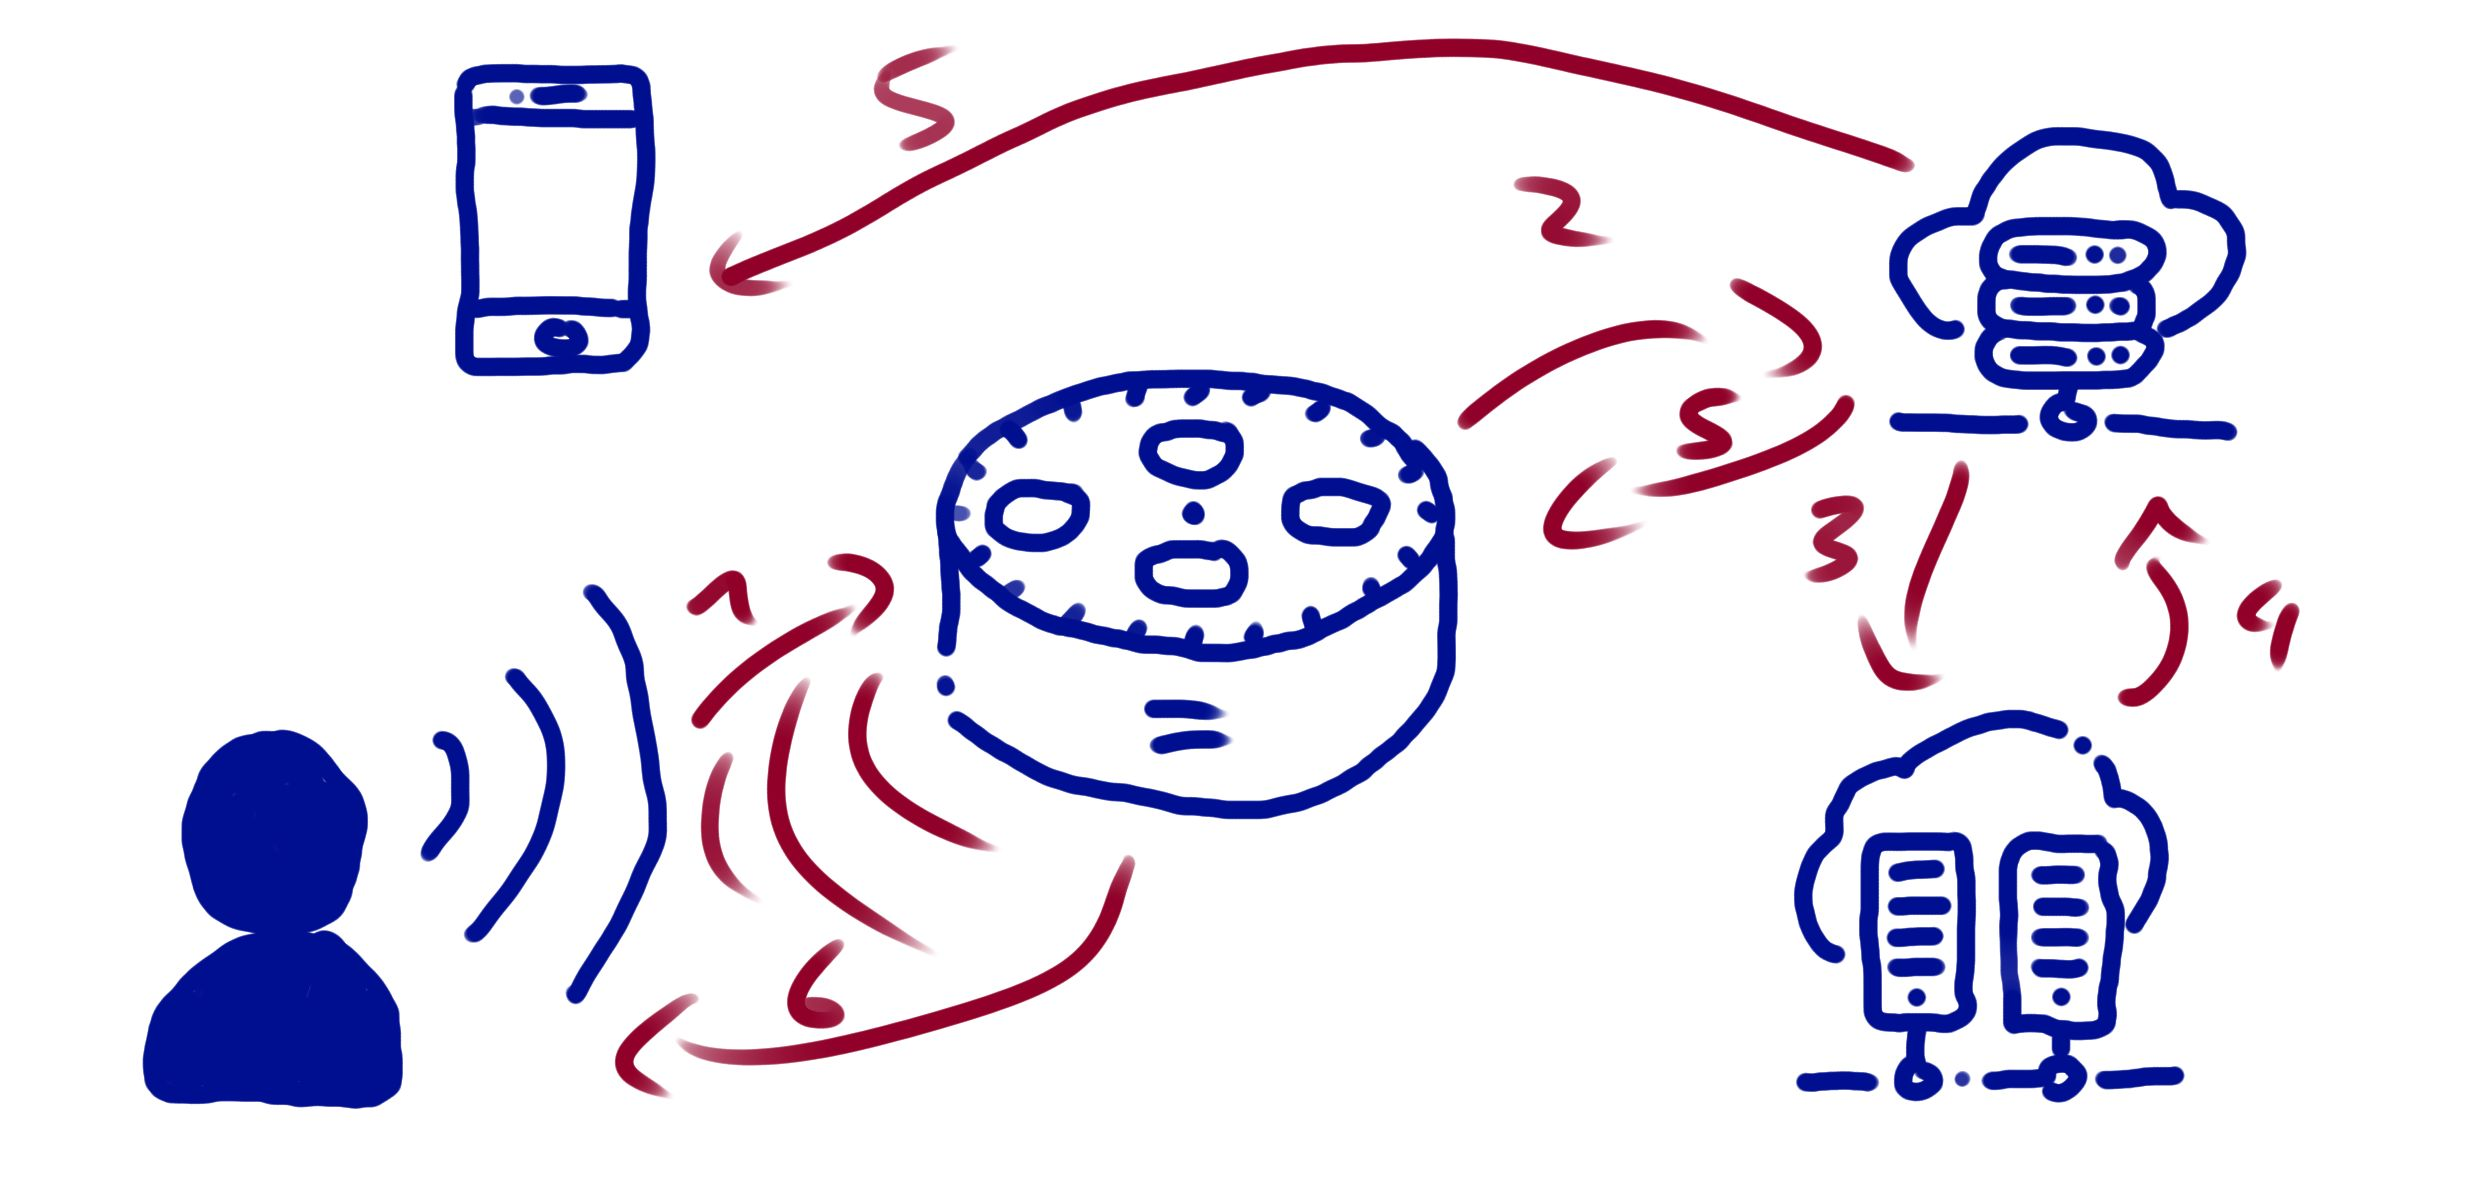
\includegraphics[width=0.9\linewidth]{images/alexatech}
\end{figure}
2. Speech Recognition on Amazon server
\end{frame}

\begin{frame}{Technology}
\begin{figure}
	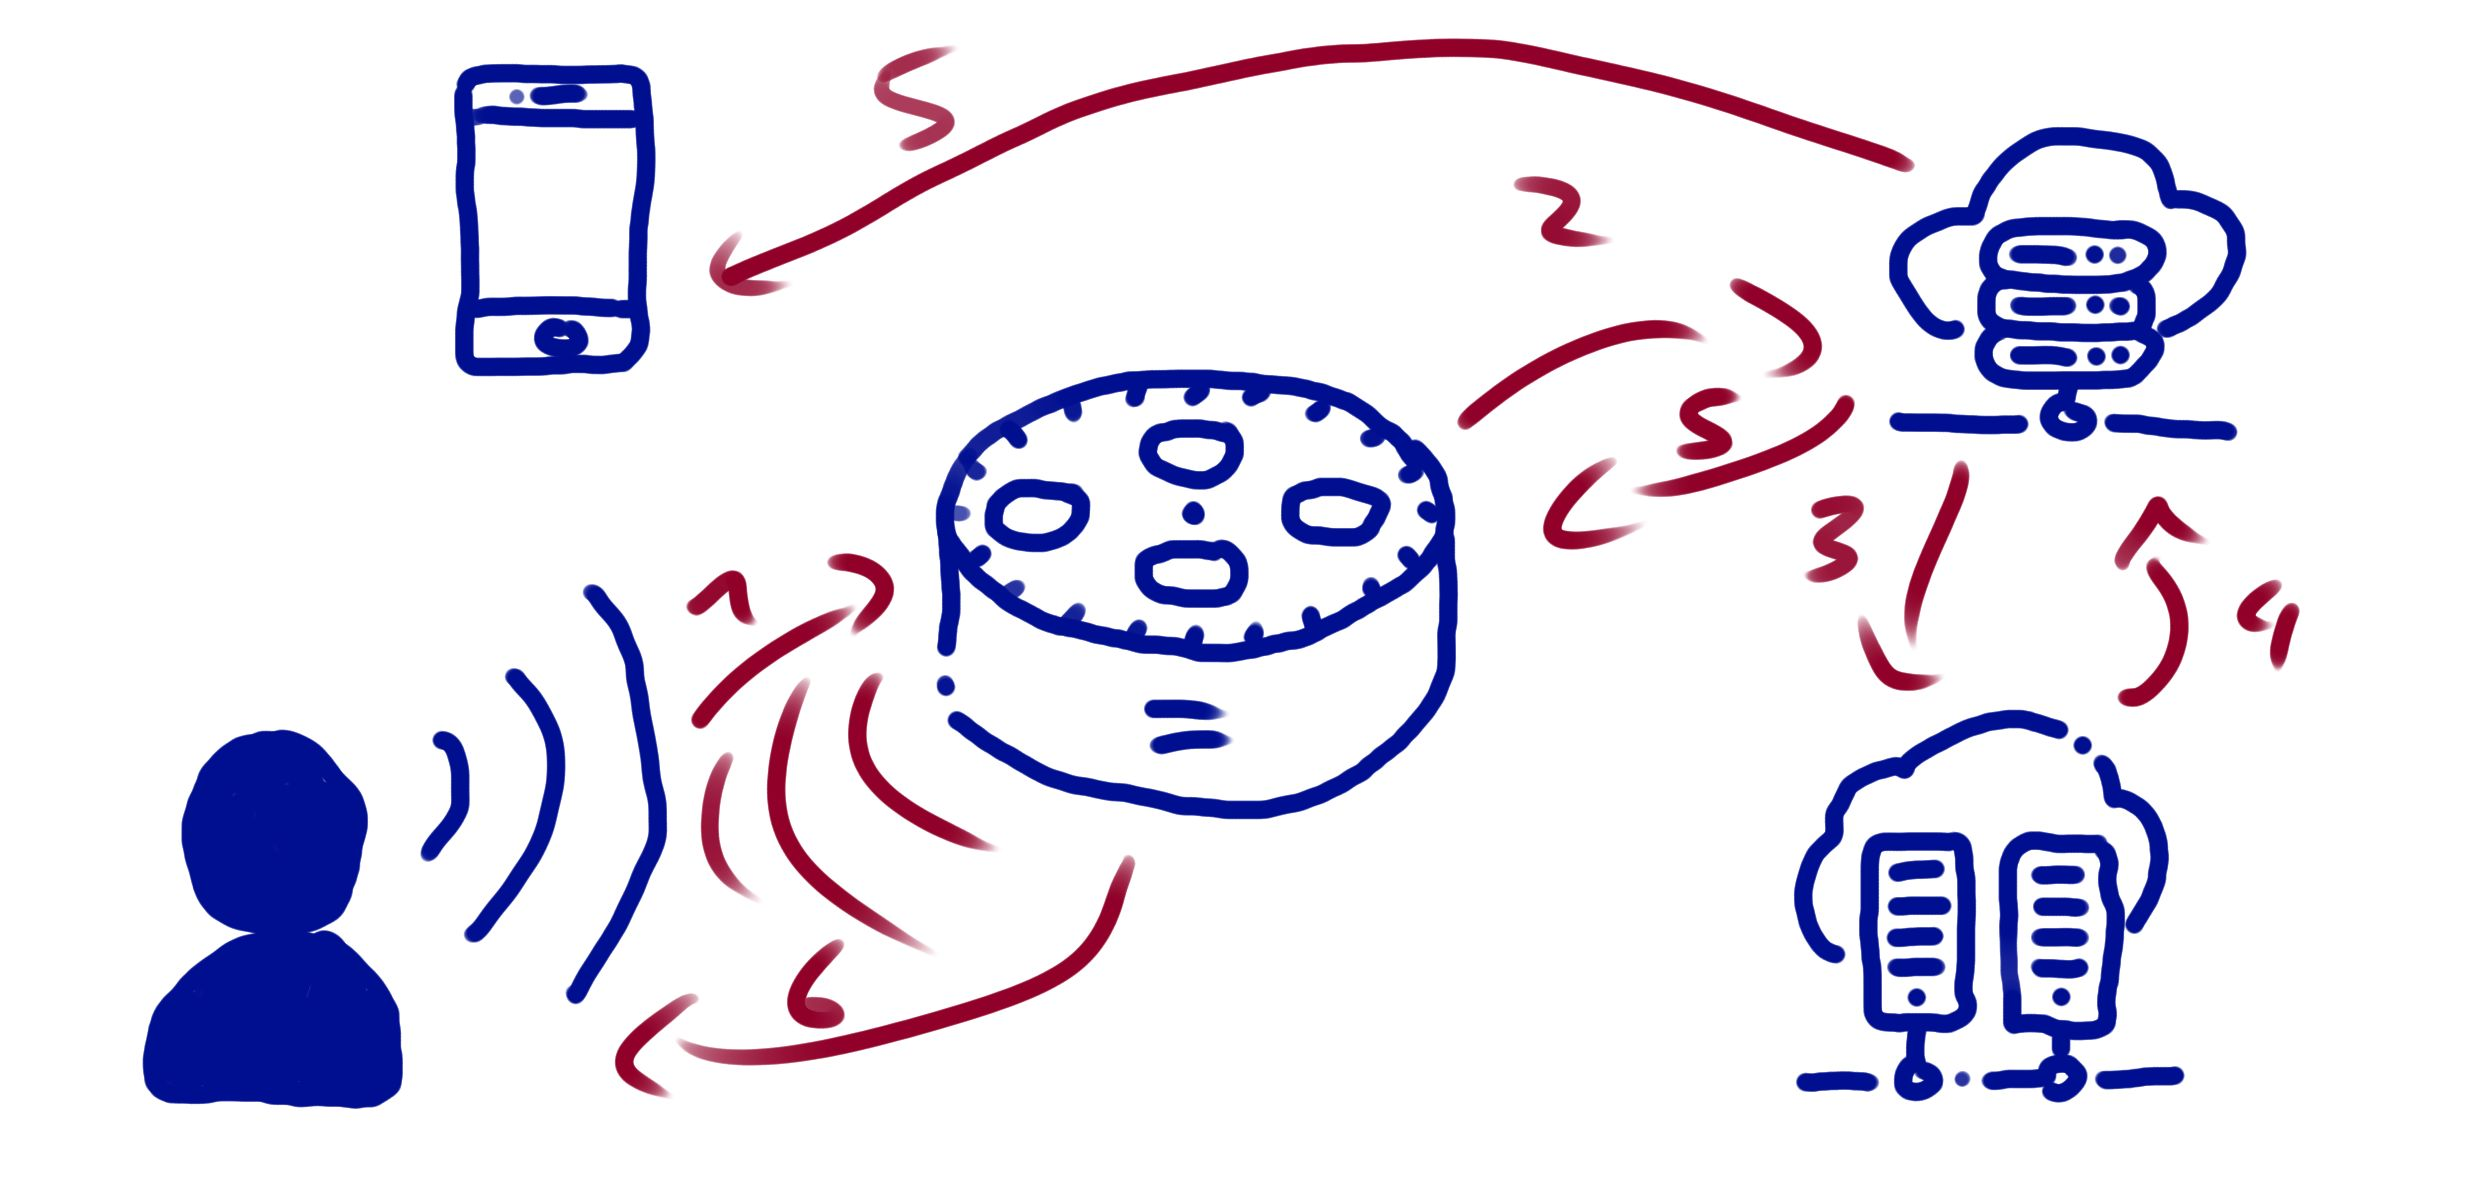
\includegraphics[width=0.9\linewidth]{images/alexatech}
\end{figure}
3. Trigger Skill on publisher server
\end{frame}

\begin{frame}{Technology}
\begin{figure}
	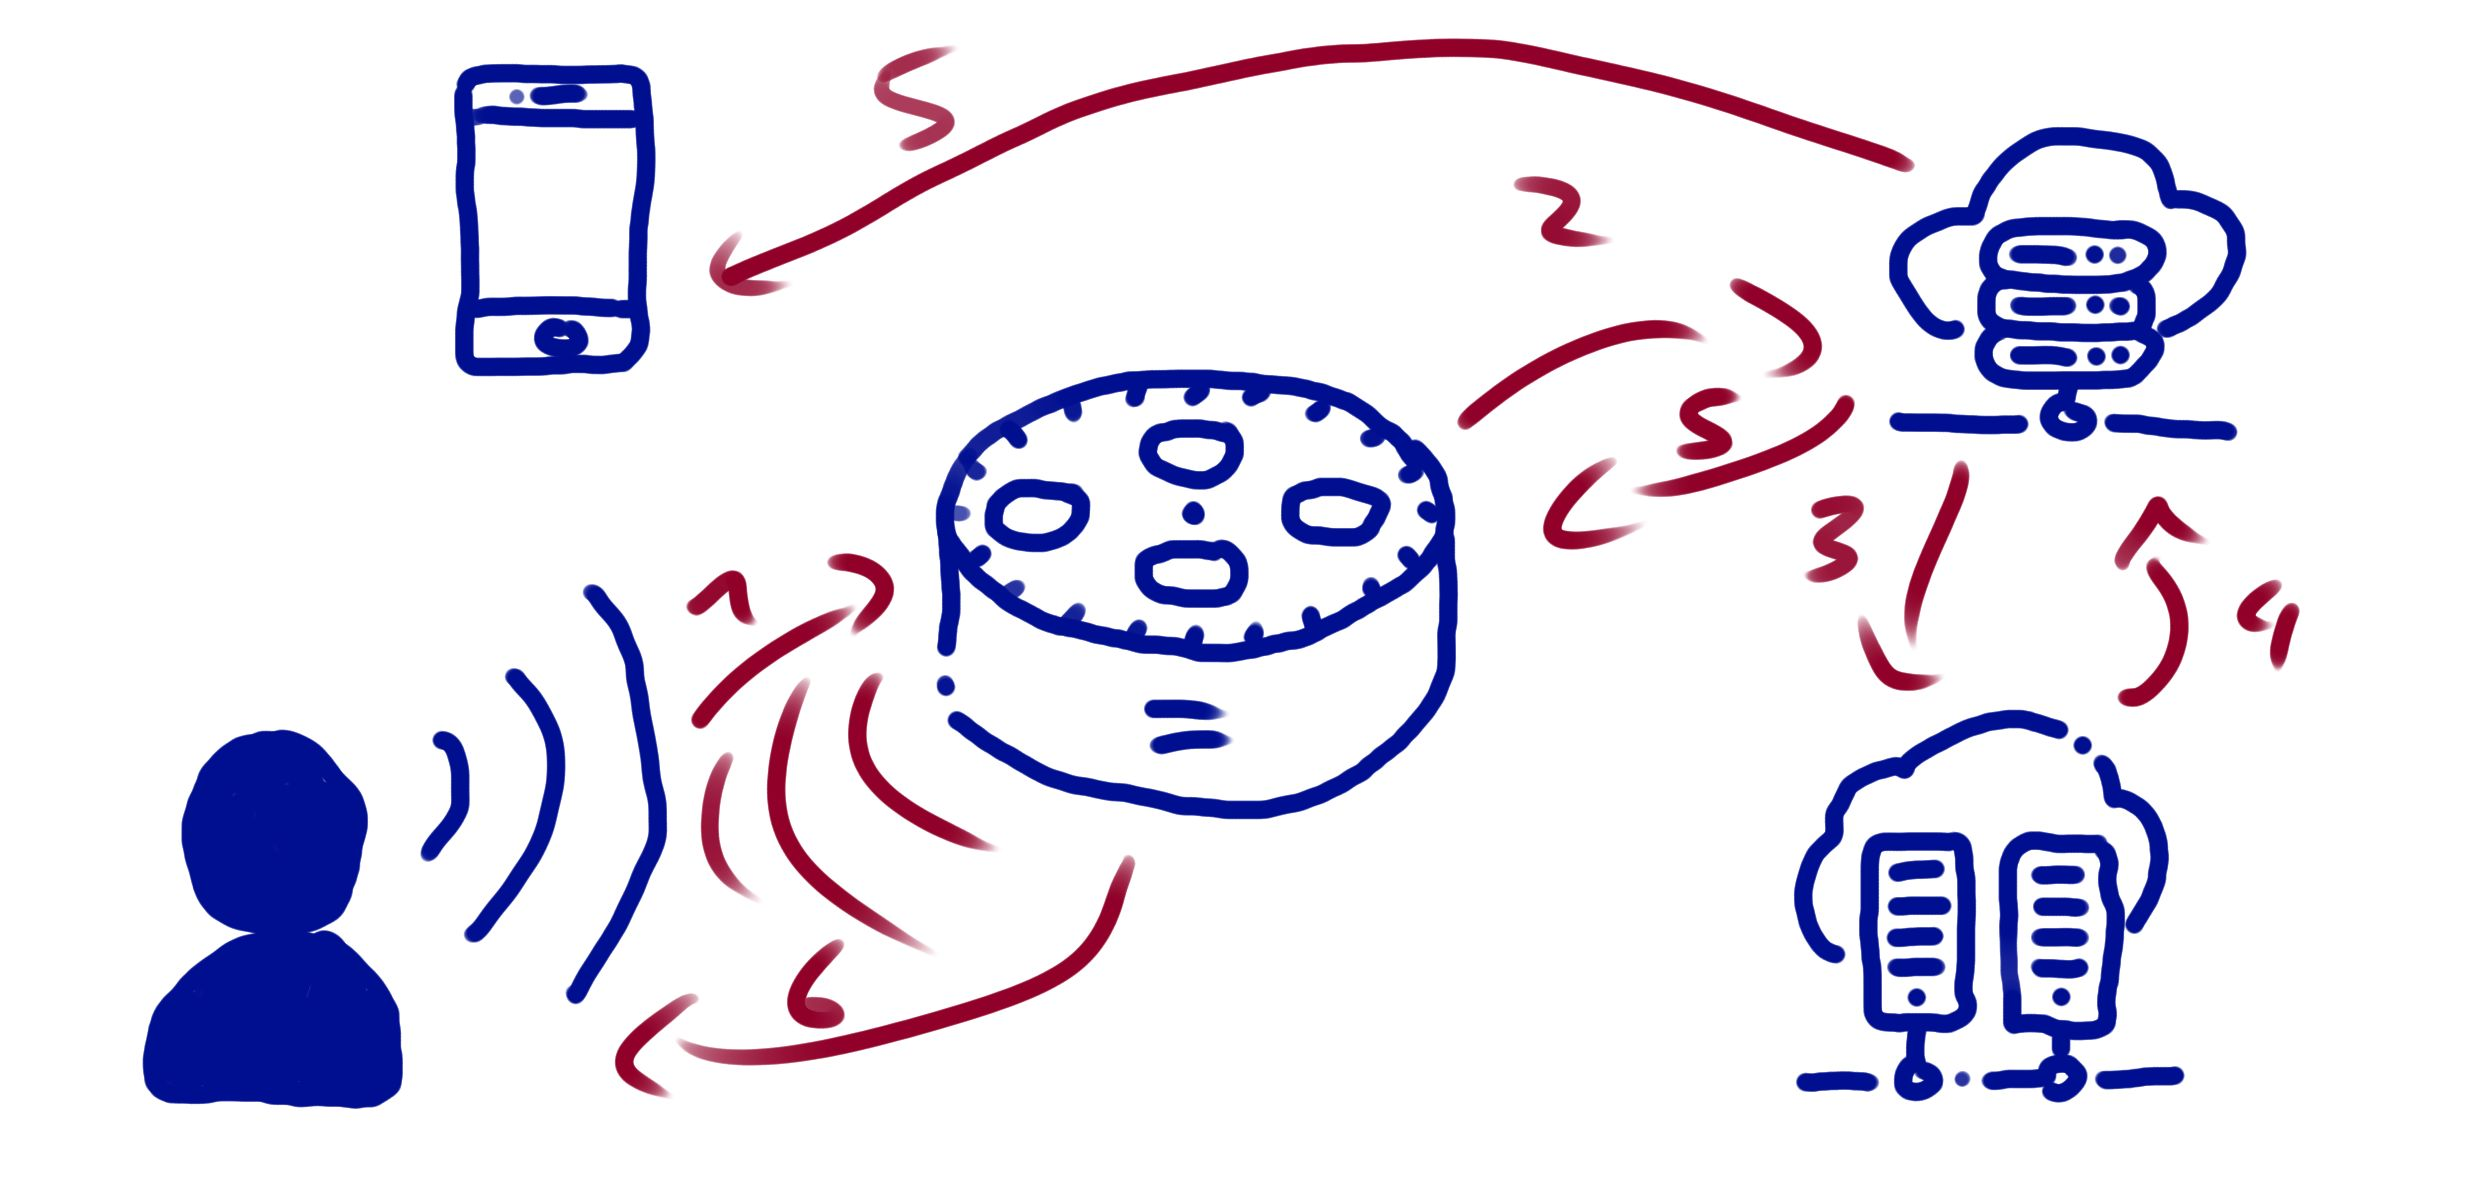
\includegraphics[width=0.9\linewidth]{images/alexatech}
\end{figure}
4. Response as Text
\end{frame}

\begin{frame}{Technology}
\begin{figure}
	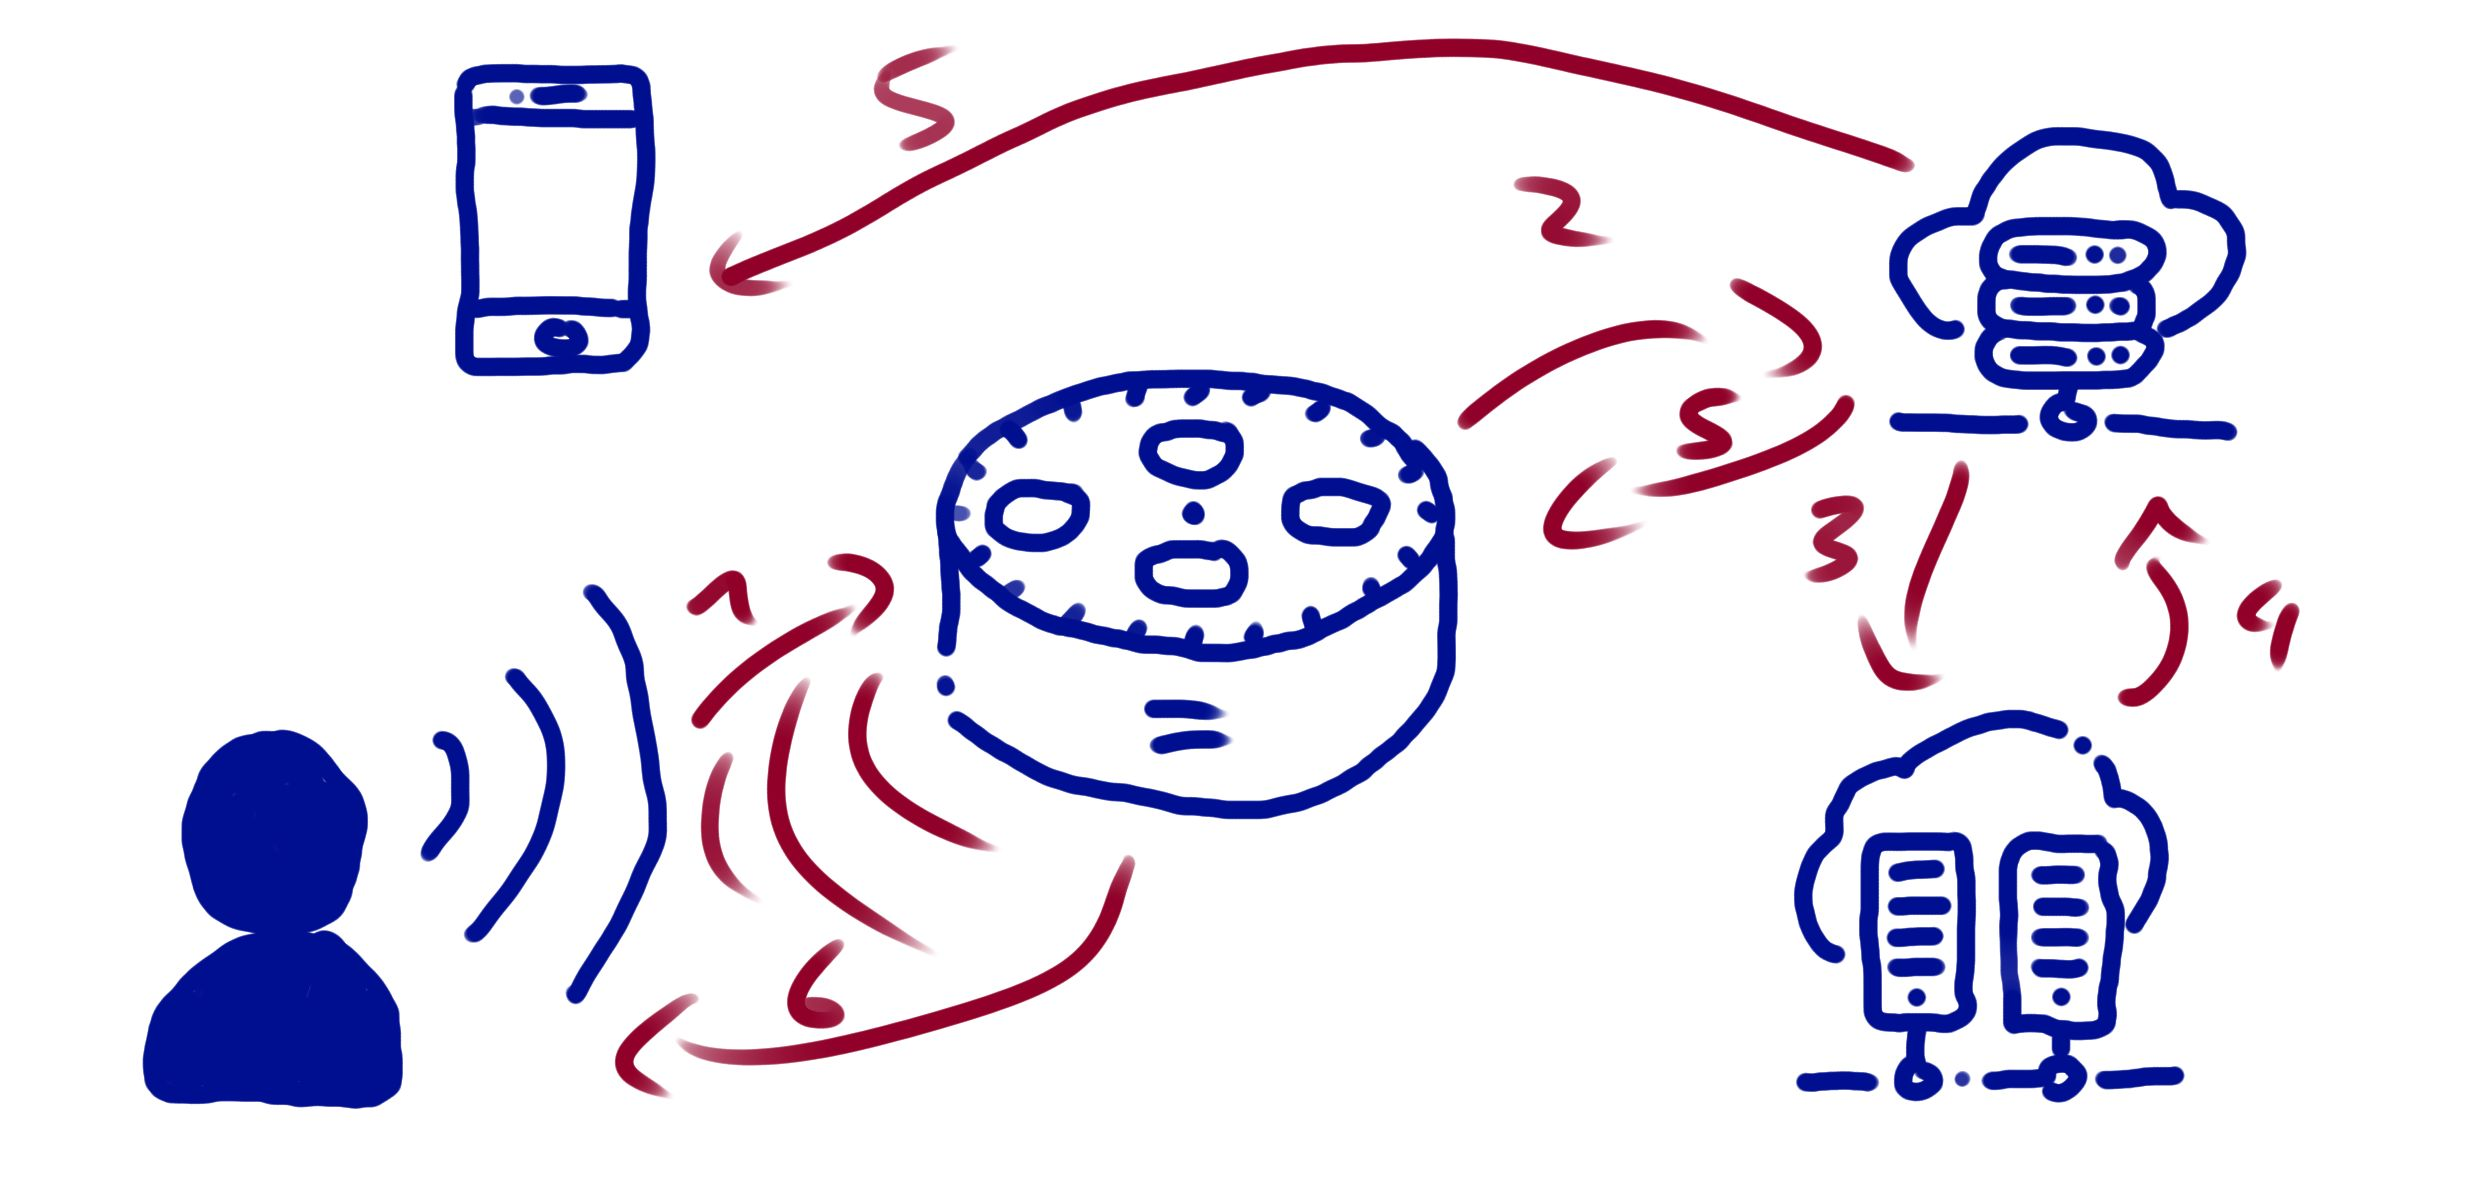
\includegraphics[width=0.9\linewidth]{images/alexatech}
\end{figure}
5. Audio Stream to Alexa, Card to Alexa App
\end{frame}

\begin{frame}{Technology}
\begin{figure}
	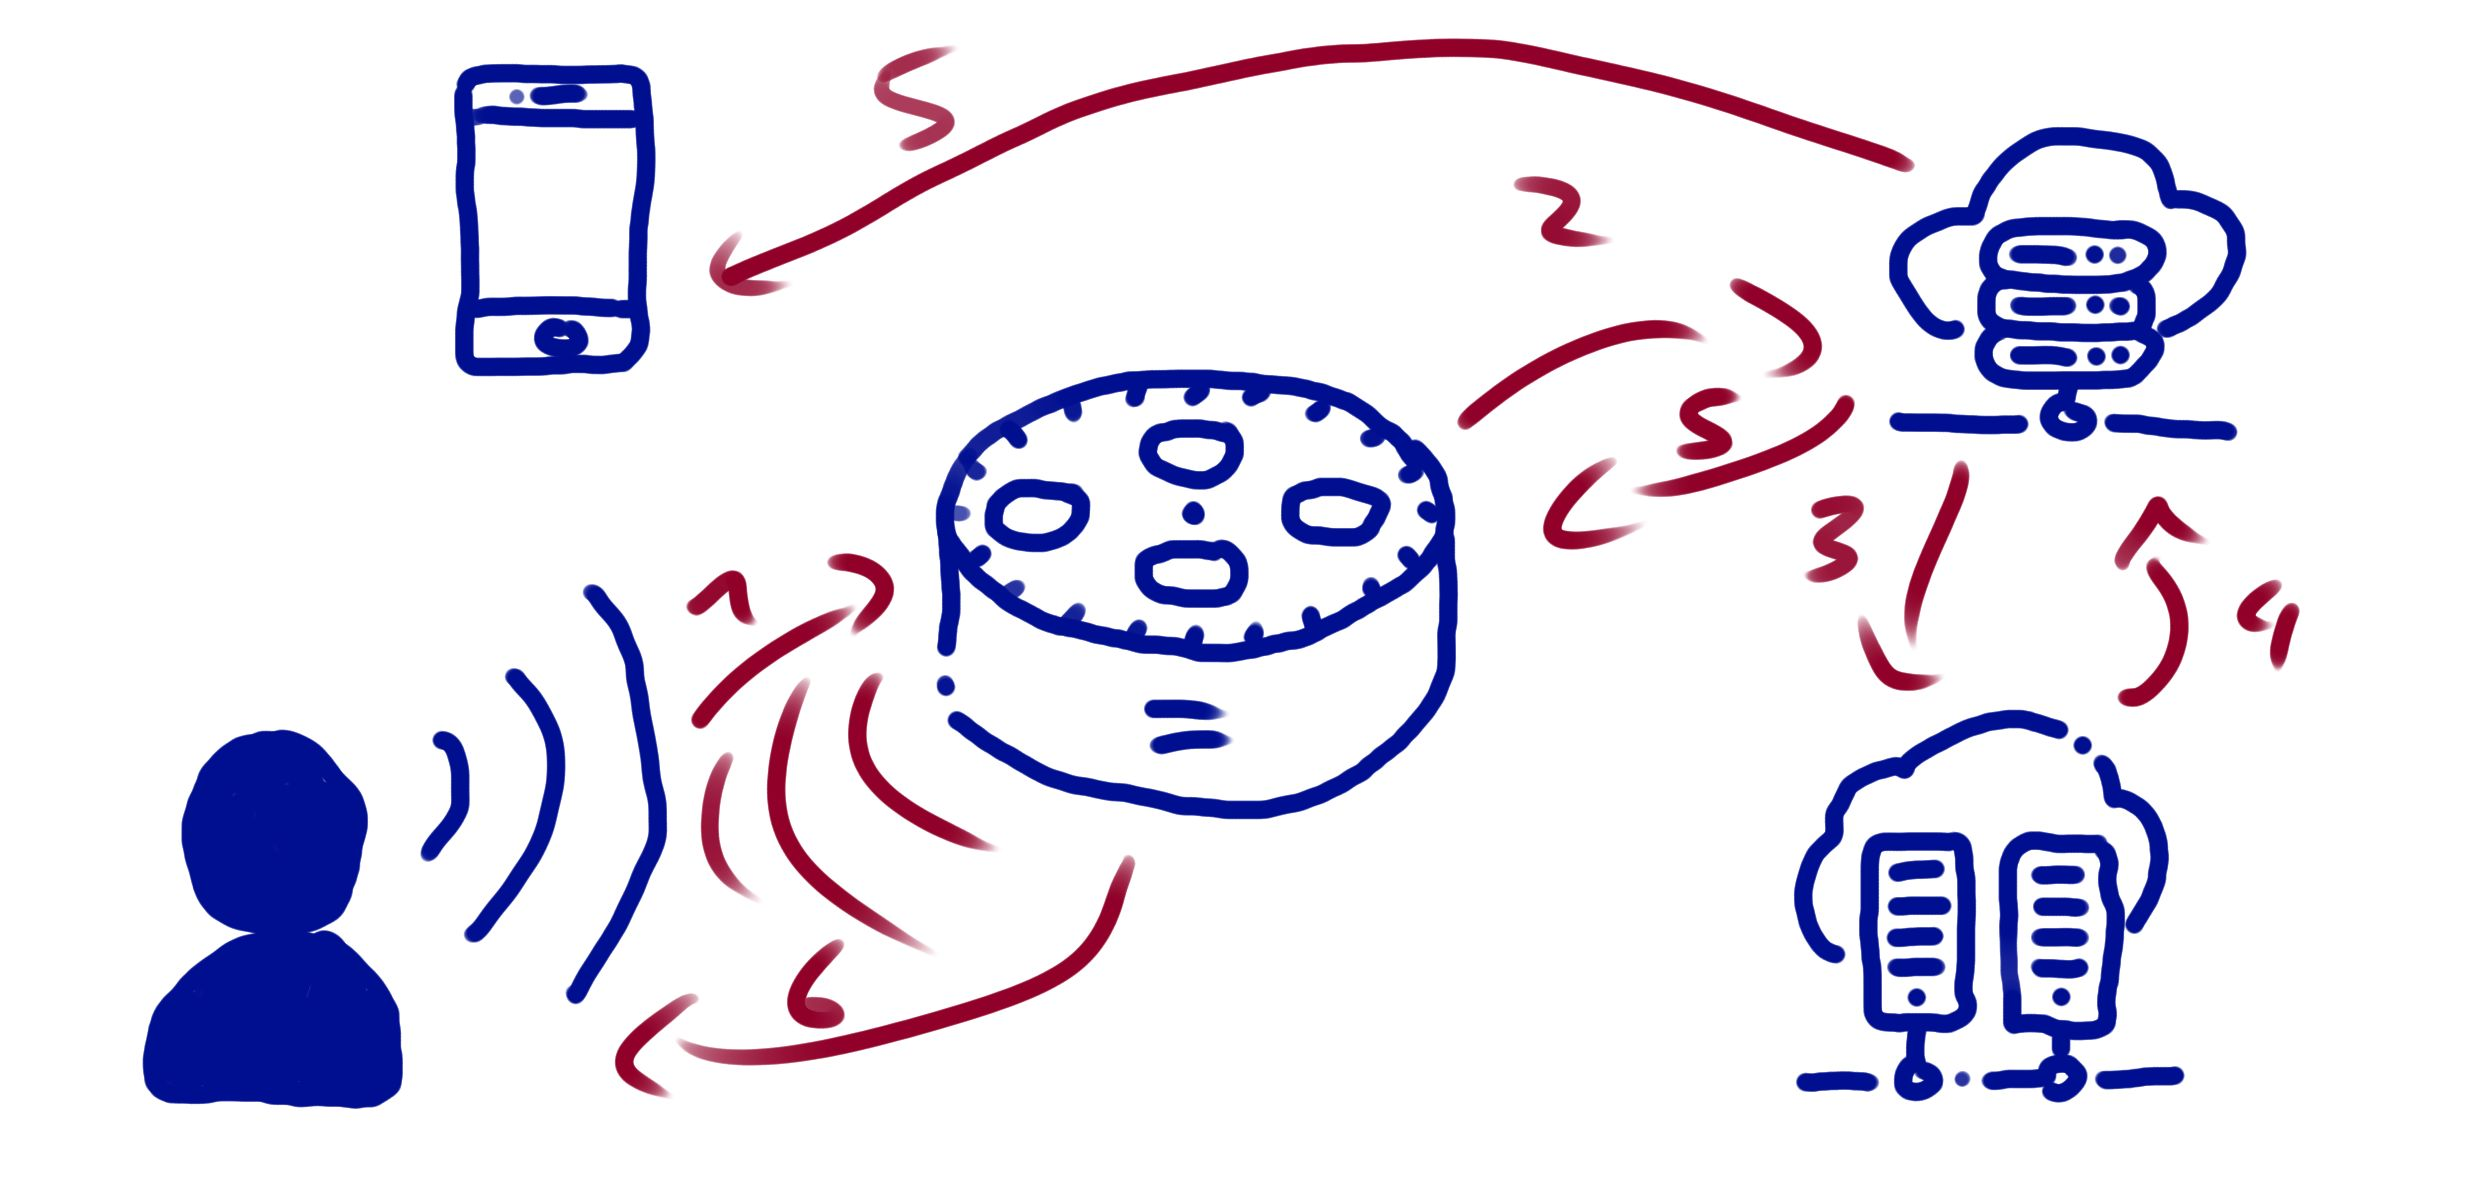
\includegraphics[width=0.9\linewidth]{images/alexatech}
\end{figure}
6. Echo plays Audio Stream
\end{frame}



\section{Workshop}
\begin{frame}{Try it yourself}
\centering
\begin{enumerate}
	\item \url{https://developer.amazon.com/alexa} $\rightarrow$ Alexa Skills Kit
	
	\item \url{https://aws.amazon.com/console/} $\rightarrow$ Lambda
	
	\item be creative
	
\end{enumerate}
\end{frame}

\begin{frame}{Discussion - End}
	\centering
	\huge{Thanks a lot for your attention!}
\end{frame}

\end{document}
